\section{Casi d'uso}
\subsection{Attori}
\begin{figure}[H]
    \centering
    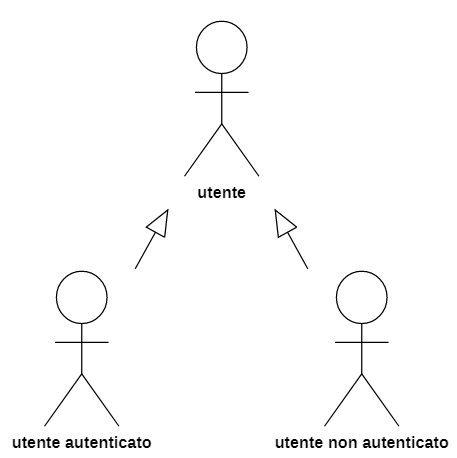
\includegraphics[width=0.5\textwidth]{res/images/utenti.png}
    \caption{Schema degli attori}
\end{figure}
\subsubsection{Utente}
Rappresenta un qualsiasi utente che sta utilizzando l’applicazione.
\paragraph{Utente non autenticato}
Rappresenta un qualsiasi utente che sta utilizzando l’applicazione senza aver effettuato l’operazione di login.
\paragraph{Utente autenticato}
Rappresenta un qualsiasi utente che sta utilizzando l’applicazione dopo aver effettuato l’operazione di login.
\subsection{Elenco casi d'uso}

Ogni caso d’uso ha un codice gerarchico ed univoco che lo identifica, nella forma:
\newline
\newline
\centerline{\textbf{UC<CodicePadre>.<CodiceFiglio>}}
\newline
\newline
Il codice progressivo può includere diversi livelli di gerarchia separati da un punto.\\

\subsubsection{UC1 - Registrazione}
\begin{figure}[H]
	\centering
	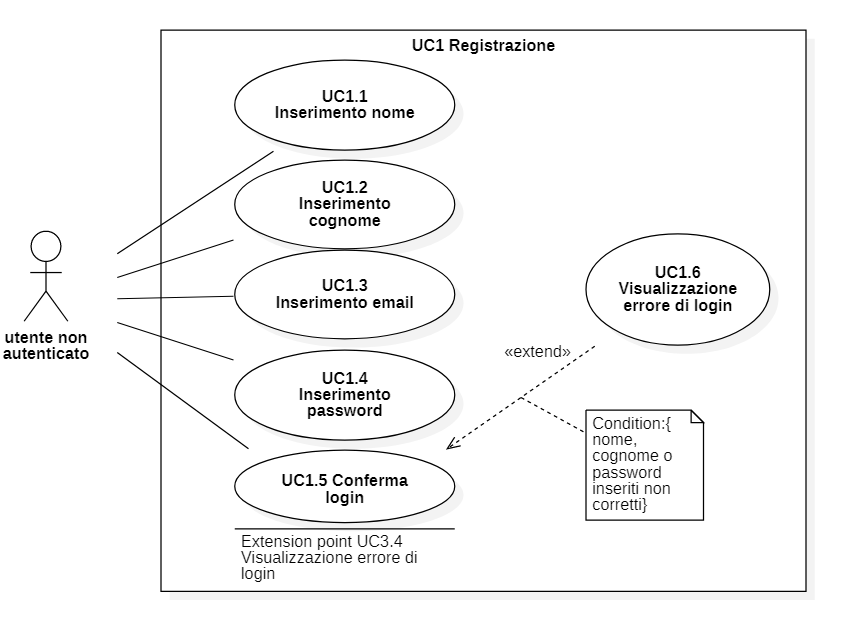
\includegraphics[width=0.8\linewidth]{res/images/UC1.png}
	\caption{Caso d'uso UC1 : registrazione}
\end{figure}
\begin{itemize}
\item \textbf{Attori}: utente non autenticato;
\item \textbf{Scopo e descrizione}: l’utente desidera registrarsi con un nuovo account inserendo dei dati personali;
\item \textbf{Precondizione}: il sito è stato caricato sul dispositivo;
\item \textbf{Flusso principale degli eventi}:
\begin{itemize}
    \item inserimento nome (UC1.1);
    \item inserimento cognome (UC1.2);
    \item inserimento email (UC1.3);
    \item inserimento password (UC1.4);
    \item conferma registrazione (UC1.5).
\end{itemize}
\item \textbf{Estensioni}:
\begin{itemize}
    \item se l’utente inserisce dei dati non validi viene visualizzato l’errore di registrazione (UC1.6 Visualizzazione errore di registrazione);
\end{itemize}
\item \textbf{Postcondizione}: l’utente inserendo i dati richiesti ha creato un nuovo account.
\end{itemize}

\subsubsection{UC1.1 - Inserimento nome utente}
\begin{itemize}
\item \textbf{Attori}: utente non autenticato;
\item \textbf{Scopo e descrizione}: l’utente deve inserire un nome per il suo account;
\item \textbf{Precondizione}: il sistema è pronto a ricevere il nome inserito dall’utente;
\item \textbf{Flusso principale degli eventi}: l’utente digita il nome;
\item \textbf{Postcondizione}: l’utente ha inserito il proprio nome nel suo account.
\end{itemize}

\subsubsection{UC1.2 - Inserimento cognome utente}
\begin{itemize}
	\item \textbf{Attori}: utente non autenticato;
	\item \textbf{Scopo e descrizione}: l’utente deve inserire un cognome identificativo del suo account;
	\item \textbf{Precondizione}: il sistema è pronto a ricevere il cognome inserito dall’utente;
	\item \textbf{Flusso principale degli eventi}: l’utente digita il cognome;
	\item \textbf{Postcondizione}: l’utente ha inserito il cognome identificativo del suo account.
\end{itemize}
\subsubsection{UC1.3 - Inserimento email}
\begin{itemize}
\item \textbf{Attori}: utente non autenticato;
\item \textbf{Scopo e descrizione}: l’utente deve inserire un indirizzo di posta elettronica che non è ancora presente nel sistema;
\item \textbf{Precondizione}: il sistema è pronto a ricevere l’email inserita dall’utente;
\item \textbf{Flusso principale degli eventi}: l’utente digita l’indirizzo di posta elettronica che desidera associare all’account;
\item \textbf{Postcondizione}: l’utente ha inserito l’email.
\end{itemize}
\subsubsection{UC1.4 - Inserimento password}
\begin{itemize}
\item \textbf{Attori}: utente non autenticato;
\item \textbf{Scopo e descrizione}: l’utente deve inserire una password con cui proteggere il proprio account. Il sistema deve nascondere alla vista i caratteri inseriti, sostituendoli con dei segnaposto;
\item \textbf{Precondizione}: il sistema è pronto a ricevere una password inserita dall’utente;
\item \textbf{Flusso principale degli eventi}: l’utente digita la password desiderata;
\item \textbf{Postcondizione}: l’utente ha inserito la password di protezione del suo account.
\end{itemize}
\subsubsection{UC1.5 - Conferma registrazione}
\begin{itemize}
\item \textbf{Attori}: utente non autenticato;
\item \textbf{Scopo e descrizione}: l’utente deve confermare i dati inseriti durante la fase di registrazione;
\item \textbf{Precondizione}: il sistema mostra una schermata che permette all’utente di confermare i dati inseriti;
\item \textbf{Flusso principale degli eventi}: l’utente conferma i dati inseriti;
\item \textbf{Postcondizione}: l’utente ha confermato i dati inseriti e il sistema ha creato un account con tali informazioni.
\end{itemize}
\subsubsection{UC1.6 - Visualizzazione errore di registrazione}
\begin{itemize}
\item \textbf{Attori}: utente non autenticato;
\item \textbf{Scopo e descrizione}: l’utente ha inserito durante la fase di registrazione dei dati non validi. Essi possono essere: campi vuoti, l’email è già collegata ad un altro account o non è valida, la password non soddisfa i requisiti di sicurezza;
\item \textbf{Precondizione}: l’utente ha inserito dei dati non validi per la creazione di un account;
\item \textbf{Flusso principale degli eventi}: il sistema mostra a schermo un errore di registrazione;
\item \textbf{Postcondizione}: l’account non viene creato e viene comunicato il messaggio di errore all’utente.
\end{itemize}

\subsubsection{UC2 - Login}
\begin{figure}[H]
    \centering
    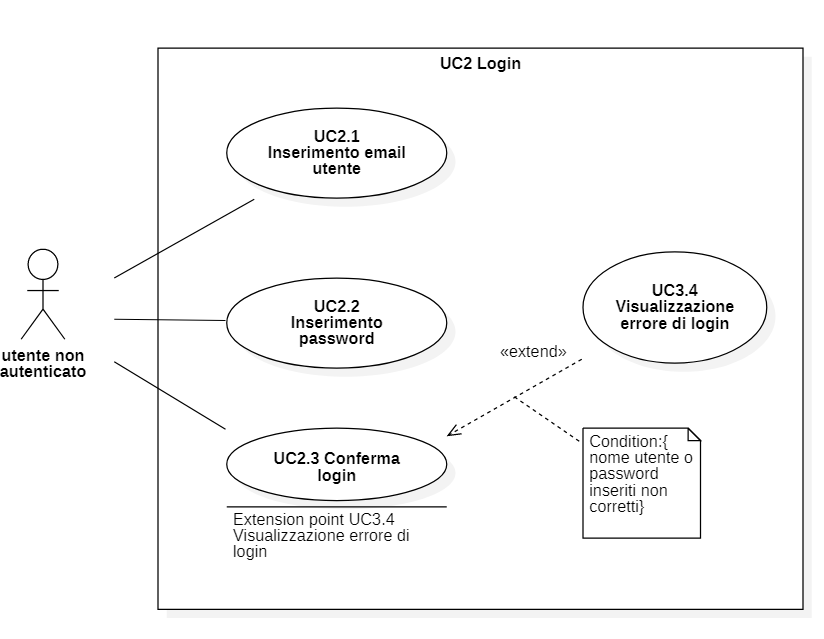
\includegraphics[width=0.8\textwidth]{res/images/UC2.png}
    \caption{Caso d'uso UC2 : Login}
\end{figure}
\begin{itemize}
\item \textbf{Attori}: utente non autenticato;
\item \textbf{Scopo e descrizione}: l’utente desidera effettuare il login con un account esistente;
\item \textbf{Precondizione}: l’utente non ha effettuato il login nell’applicazione;
\item \textbf{Flusso principale degli eventi}:
\begin{itemize}
    \item inserimento del email utente (UC2.1);
    \item inserimento della password (UC2.2);
    \item conferma del login (UC2.3).
\end{itemize}
\item \textbf{Estensioni}: se l’utente inserisce dei dati non validi viene visualizzato l’errore di login (UC2.4);
\item \textbf{Postcondizione}: l’utente ha effettuato l’accesso con il suo account.
\end{itemize}
\subsubsection{UC2.1 - Inserimento email utente}
\begin{itemize}
\item \textbf{Attori}: utente non autenticato;
\item \textbf{Scopo e descrizione}: l’utente deve inserire l'email collegata ad un account esistente per eseguire il login;
\item \textbf{Precondizione}: il sistema è pronto a ricevere l'email inserita dall’utente;
\item \textbf{Flusso principale degli eventi}: l’utente digita l'email desiderata;
\item \textbf{Postcondizione}: l’utente ha inserito il nome identificativo di un account.
\end{itemize}
\subsubsection{UC2.2 - Inserimento password}
\begin{itemize}
\item \textbf{Attori}: utente non autenticato;
\item \textbf{Scopo e descrizione}: l’utente deve inserire la password di accesso del suo account per eseguire il login;
\item \textbf{Precondizione}: il sistema è pronto a ricevere la password dell’utente;
\item \textbf{Flusso principale degli eventi}: l’utente digita la propria password che viene visualizzata sostituendo i caratteri con dei segnaposto;
\item \textbf{Postcondizione}: l’utente ha inserito la password del suo account.
\end{itemize}
\subsubsection{UC2.3 - Conferma login}
\begin{itemize}
\item \textbf{Attori}: utente non autenticato;
\item \textbf{Scopo e descrizione}: l’utente intende confermare i dati inseriti per procedere con il login;
\item \textbf{Precondizione}: il sistema mostra una schermata che permette all’utente di confermare i dati inseriti;
\item \textbf{Flusso principale degli eventi}: l’utente conferma i dati inseriti;
\item \textbf{Postcondizione}: l’utente ha eseguito l’accesso al proprio account.
\end{itemize}
\subsubsection{UC2.4 - Visualizzazione errore login}
\begin{itemize}
\item \textbf{Attori}: utente non autenticato;
\item \textbf{Scopo e descrizione}: l’utente ha inserito durante la fase di login dei dati non validi. Essi possono essere: l'email non è presente nel sistema, la password non è corretta;
\item \textbf{Precondizione}: l’utente ha inserito dei dati non validi per il login;
\item \textbf{Flusso principale degli eventi}: il sistema mostra a schermo un errore di autenticazione;
\item \textbf{Postcondizione}: l’account non viene collegato e viene comunicato il messaggio di errore all’utente.
\end{itemize}
\subsubsection{UC3 - Logout}
\begin{itemize}
\item \textbf{Attori}: utente autenticato;
\item \textbf{Scopo e descrizione}: l’utente desidera scollegare il suo account dal dispositivo;
\item \textbf{Precondizione}: l’utente ha precedentemente effettuato il login nel sito;
\item \textbf{Flusso principale degli eventi}: l’utente dichiara di voler effettuare il logout;
\item \textbf{Postcondizione}: l’utente ha effettuato il logout. Non è più collegato un profilo.
\end{itemize}


\subsubsection{UC4 - Visualizzazione elenco attività}
\begin{figure}[H]
	\centering
	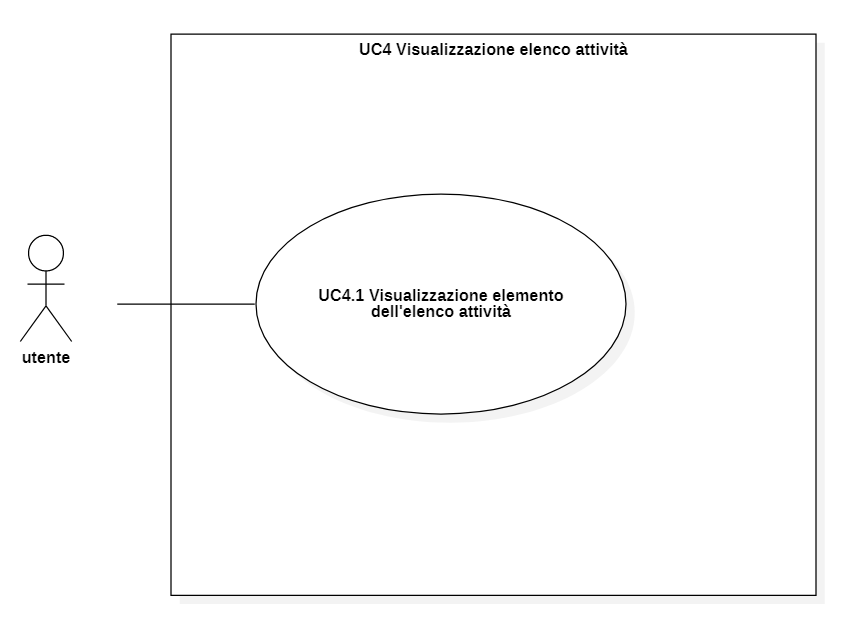
\includegraphics[width=0.8\linewidth]{res/images/UC4.png}
	\caption{Caso d'uso UC4 : visualizzazione elenco attività}
\end{figure}
\begin{itemize}
\item \textbf{Attori}: utente;
\item \textbf{Scopo e descrizione}: l’utente visualizza l'elenco delle attività sportive disponibili pubblicate dagli utenti;
\item \textbf{Precondizione}: il sistema è pronto a ricevere richieste;
\item \textbf{Flusso principale degli eventi}:visualizzazione elemento dell'elenco attività(UC4.1);
\item \textbf{Postcondizione}: il sistema ha mostrato a schermo l'elenco delle attività.
\end{itemize}

\subsubsection{UC4.1 - Visualizzazione elemento dell'elenco attività}
\begin{figure}[H]
	\centering
	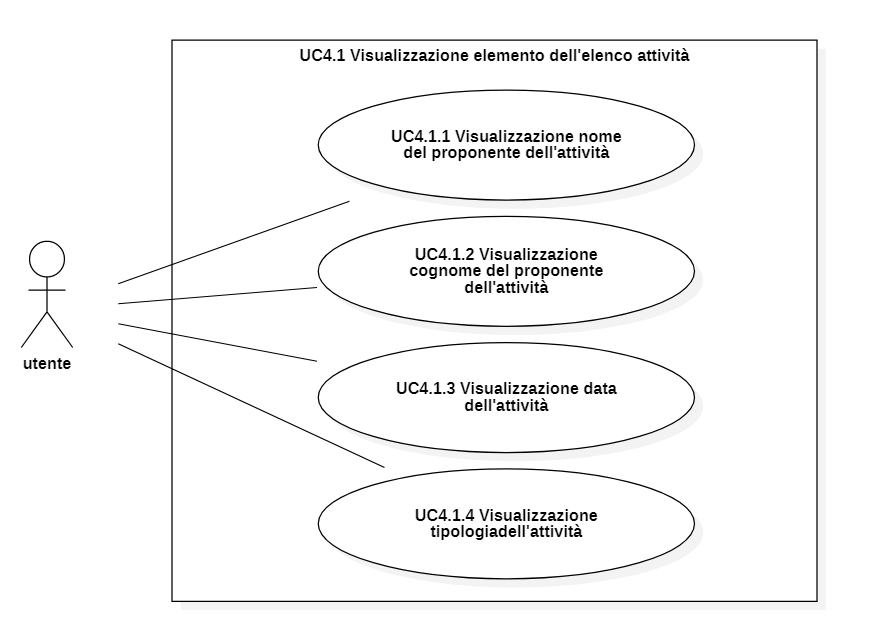
\includegraphics[width=0.8\linewidth]{res/images/UC4.1.png}
	\caption{Caso d'uso UC4.1 : visualizzazione elemento dell'elenco attività}
\end{figure}
\begin{itemize}
\item \textbf{Attori}: utente;
\item \textbf{Scopo e descrizione}: l’utente vuole prendere visione di un elemento dell'elenco;
\item \textbf{Precondizione}: il sistema ha precedentemente memorizzato ed elaborato i dati relativi all'attività;
\item \textbf{Flusso principale degli eventi}:
\begin{itemize}
    \item visualizzazione nome del proponente dell’attività (UC4.1.1);
    \item visualizzazione cognome del proponente dell’attività (UC4.1.2);
    \item visualizzazione data dell’attività (UC4.1.3);
    \item visualizzazione tipologia dell’attività (UC4.1.4).
\end{itemize}
\item \textbf{Postcondizione}: l’utente ha visualizzato i dati correlati all’elemento dell'elenco attività.
\end{itemize}

\subsubsection{UC4.1.1 - Visualizzazione nome del proponente dell’attività }
\begin{itemize}
\item \textbf{Attori}: utente;
\item \textbf{Scopo e descrizione}: l’utente vuole prendere visione del nome dell'utente che ha proposto l'attività;
\item \textbf{Precondizione}: il sistema ha in memoria il nome dell'utente proponente dell'attività;
\item \textbf{Flusso principale degli eventi}: il sistema mostra il nome;
\item \textbf{Postcondizione}: l’utente ha visualizzato il nome del proponente dell’attività.
\end{itemize}

\subsubsection{UC4.1.2 - Visualizzazione cognome del proponente dell’attività }
\begin{itemize}
	\item \textbf{Attori}: utente;
	\item \textbf{Scopo e descrizione}: l’utente vuole prendere visione del cognome dell'utente che ha proposto l'attività;
	\item \textbf{Precondizione}: il sistema ha in memoria il cognome dell'utente proponente dell'attività;
	\item \textbf{Flusso principale degli eventi}: il sistema mostra il cognome;
	\item \textbf{Postcondizione}: l’utente ha visualizzato il cognome del proponente dell’attività.
\end{itemize}

\subsubsection{UC4.1.3 - Visualizzazione data dell’attività }
\begin{itemize}
	\item \textbf{Attori}: utente;
	\item \textbf{Scopo e descrizione}: l’utente vuole prendere visione della data dell'attività;
	\item \textbf{Precondizione}: il sistema ha in memoria la data dell'attività;
	\item \textbf{Flusso principale degli eventi}: il sistema mostra la data dell'attività;
	\item \textbf{Postcondizione}: l’utente ha visualizzato la data dell'attività.
\end{itemize}

\subsubsection{UC4.1.4 - Visualizzazione tipologia dell’attività }
\begin{itemize}
	\item \textbf{Attori}: utente;
	\item \textbf{Scopo e descrizione}: l’utente vuole prendere visione della tipologia dell’attività;
	\item \textbf{Precondizione}: il sistema ha in memoria la tipologia dell’attività;
	\item \textbf{Flusso principale degli eventi}: il sistema mostra la tipologia dell’attività;
	\item \textbf{Postcondizione}: l’utente ha visualizzato la tipologia dell’attività.
\end{itemize}


\subsubsection{UC5 - Visualizzazione dettaglio di un'attività}
\begin{figure}[H]
	\centering
	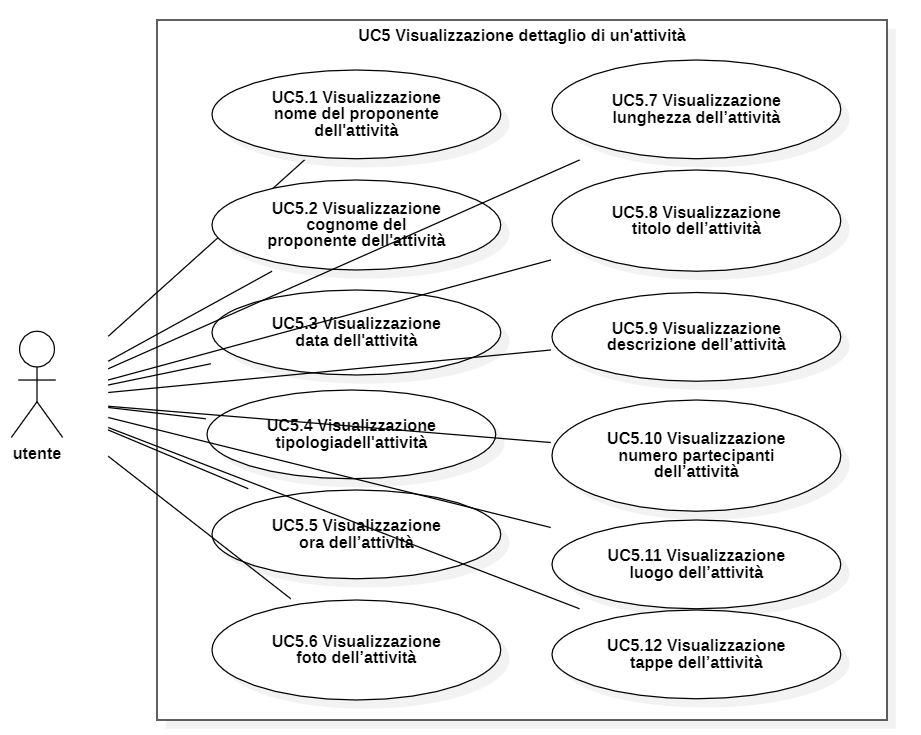
\includegraphics[width=0.8\linewidth]{res/images/UC5.png}
	\caption{Caso d'uso UC5 : visualizzazione dettaglio di un'attività}
\end{figure}
\begin{itemize}
	\item \textbf{Attori}: utente;
	\item \textbf{Scopo e descrizione}: l’utente vuole prendere visione dei dettagli di un'attività;
	\item \textbf{Precondizione}: l'utente ha selezionato quella attività e il sistema ha precedentemente memorizzato ed elaborato i dati relativi a tale attività;
	\item \textbf{Flusso principale degli eventi}:
	\begin{itemize}
		\item visualizzazione nome del proponente dell’attività (UC5.1);
		\item visualizzazione cognome del proponente  dell’attività (UC5.2);
		\item visualizzazione data dell’attività (UC5.3);
		\item visualizzazione tipologia dell’attività (UC5.4);
		\item visualizzazione ora dell’attività (UC5.5);
		\item visualizzazione foto dell’attività (UC5.6);
		\item visualizzazione lunghezza dell’attività (UC5.7);
		\item visualizzazione titolo dell’attività (UC5.8);
		\item visualizzazione descrizione dell’attività (UC5.9);
		\item visualizzazione numero partecipanti dell’attività (UC5.10);
		\item visualizzazione luogo dell’attività (UC5.11);
		\item visualizzazione tappe dell’attività (UC5.12).
	\end{itemize}
	\item \textbf{Postcondizione}: l’utente ha visualizzato i dati di un'attività.
\end{itemize}


\subsubsection{UC5.1 - Visualizzazione nome del proponente dell’attività }
\begin{itemize}
	\item \textbf{Attori}: utente;
	\item \textbf{Scopo e descrizione}: l’utente vuole prendere visione del nome dell'utente che ha proposto l'attività selezionata;
	\item \textbf{Precondizione}: il sistema ha in memoria il nome dell'utente proponente dell'attività;
	\item \textbf{Flusso principale degli eventi}: il sistema mostra il nome;
	\item \textbf{Postcondizione}: l’utente ha visualizzato il nome del proponente dell’attività.
\end{itemize}

\subsubsection{UC5.2 - Visualizzazione cognome del proponente dell’attività }
\begin{itemize}
	\item \textbf{Attori}: utente;
	\item \textbf{Scopo e descrizione}: l’utente vuole prendere visione del cognome dell'utente che ha proposto l'attività selezionata;
	\item \textbf{Precondizione}: il sistema ha in memoria il cognome dell'utente proponente dell'attività;
	\item \textbf{Flusso principale degli eventi}: il sistema mostra il cognome;
	\item \textbf{Postcondizione}: l’utente ha visualizzato il cognome del proponente dell’attività.
\end{itemize}

\subsubsection{UC5.3 - Visualizzazione data dell’attività }
\begin{itemize}
	\item \textbf{Attori}: utente;
	\item \textbf{Scopo e descrizione}: l’utente vuole prendere visione della data dell'attività selezionata;
	\item \textbf{Precondizione}: il sistema ha in memoria la data dell'attività;
	\item \textbf{Flusso principale degli eventi}: il sistema mostra la data dell'attività;
	\item \textbf{Postcondizione}: l’utente ha visualizzato la data dell'attività.
\end{itemize}

\subsubsection{UC5.4- Visualizzazione tipologia dell’attività }
\begin{itemize}
	\item \textbf{Attori}: utente;
	\item \textbf{Scopo e descrizione}: l’utente vuole prendere visione della tipologia dell’attività selezionata;
	\item \textbf{Precondizione}: il sistema ha in memoria la tipologia dell’attività;
	\item \textbf{Flusso principale degli eventi}: il sistema mostra la tipologia dell’attività;
	\item \textbf{Postcondizione}: l’utente ha visualizzato la tipologia dell’attività.
\end{itemize}

\subsubsection{UC5.5 - Visualizzazione ora dell’attività }
\begin{itemize}
	\item \textbf{Attori}: utente;
	\item \textbf{Scopo e descrizione}: l’utente vuole prendere visione dell'ora di inizio dell'attività selezionata;
	\item \textbf{Precondizione}: il sistema ha in memoria l'ora di inizio dell'attività;
	\item \textbf{Flusso principale degli eventi}: il sistema mostra l'ora;
	\item \textbf{Postcondizione}: l’utente ha visualizzato l'ora di inizio dell’attività.
\end{itemize}

\subsubsection{UC5.6 - Visualizzazione foto dell’attività }
\begin{itemize}
	\item \textbf{Attori}: utente;
	\item \textbf{Scopo e descrizione}: l’utente vuole prendere visione della foto raffigurante l'attività selezionata;
	\item \textbf{Precondizione}: il sistema ha in memoria la foto dell'attività;
	\item \textbf{Flusso principale degli eventi}: il sistema mostra la foto;
	\item \textbf{Postcondizione}: l’utente ha visualizzato la foto dell’attività.
\end{itemize}

\subsubsection{UC5.7 - Visualizzazione lunghezza dell’attività }
\begin{itemize}
	\item \textbf{Attori}: utente;
	\item \textbf{Scopo e descrizione}: l’utente vuole prendere visione della lunghezza in km dell'attività selezionata;
	\item \textbf{Precondizione}: il sistema ha in memoria la lunghezza dell'attività;
	\item \textbf{Flusso principale degli eventi}: il sistema mostra la lunghezza dell'attività;
	\item \textbf{Postcondizione}: l’utente ha visualizzato la lunghezza dell'attività.
\end{itemize}

\subsubsection{UC5.8 - Visualizzazione titolo dell’attività }
\begin{itemize}
	\item \textbf{Attori}: utente;
	\item \textbf{Scopo e descrizione}: l’utente vuole prendere visione del titolo dell’attività selezionata;
	\item \textbf{Precondizione}: il sistema ha in memoria il titolo dell’attività;
	\item \textbf{Flusso principale degli eventi}: il sistema mostra il titolo dell’attività;
	\item \textbf{Postcondizione}: l’utente ha visualizzato il titolo dell’attività.
\end{itemize}

\subsubsection{UC5.9 - Visualizzazione descrizione dell’attività }
\begin{itemize}
	\item \textbf{Attori}: utente;
	\item \textbf{Scopo e descrizione}: l’utente vuole prendere visione della descrizione dell'attività selezionata;
	\item \textbf{Precondizione}: il sistema ha in memoria la descrizione dell'attività;
	\item \textbf{Flusso principale degli eventi}: il sistema mostra la descrizione dell'attività;
	\item \textbf{Postcondizione}: l’utente ha visualizzato la descrizione dell'attività;
\end{itemize}

\subsubsection{UC5.10 - Visualizzazione numero partecipanti dell’attività }
\begin{itemize}
	\item \textbf{Attori}: utente;
	\item \textbf{Scopo e descrizione}: l’utente vuole prendere visione del numero dei partecipanti all'attività selezionata;
	\item \textbf{Precondizione}: il sistema ha in memoria il numero dei partecipanti all'attività;
	\item \textbf{Flusso principale degli eventi}: il sistema mostra numero dei partecipanti;
	\item \textbf{Postcondizione}: l’utente ha visualizzato il numero dei partecipanti all'attività.
\end{itemize}
\subsubsection{UC5.11 - Visualizzazione luogo dell’attività }
\begin{itemize}
	\item \textbf{Attori}: utente;
	\item \textbf{Scopo e descrizione}: l’utente vuole prendere visione del luogo in si svolge dell’attività selezionata;
	\item \textbf{Precondizione}: il sistema ha in memoria il luogo dell’attività;
	\item \textbf{Flusso principale degli eventi}: il sistema mostra il luogo dell’attività;
	\item \textbf{Postcondizione}: l’utente ha visualizzato il luogo dell’attività.
\end{itemize}
\subsubsection{UC5.12 - Visualizzazione tappe dell’attività }
\begin{itemize}
	\item \textbf{Attori}: utente;
	\item \textbf{Scopo e descrizione}: l’utente vuole prendere visione delle tappe dell'attività selezionata;
	\item \textbf{Precondizione}: il sistema ha in memoria le tappe dell'attività;
	\item \textbf{Flusso principale degli eventi}: il sistema mostra le tappe dell'attività;
	\item \textbf{Postcondizione}: l’utente ha visualizzato le tappe dell'attività.
\end{itemize}

\subsubsection{UC6 - Visualizzazione elenco dello storico delle attività}
\begin{figure}[H]
	\centering
	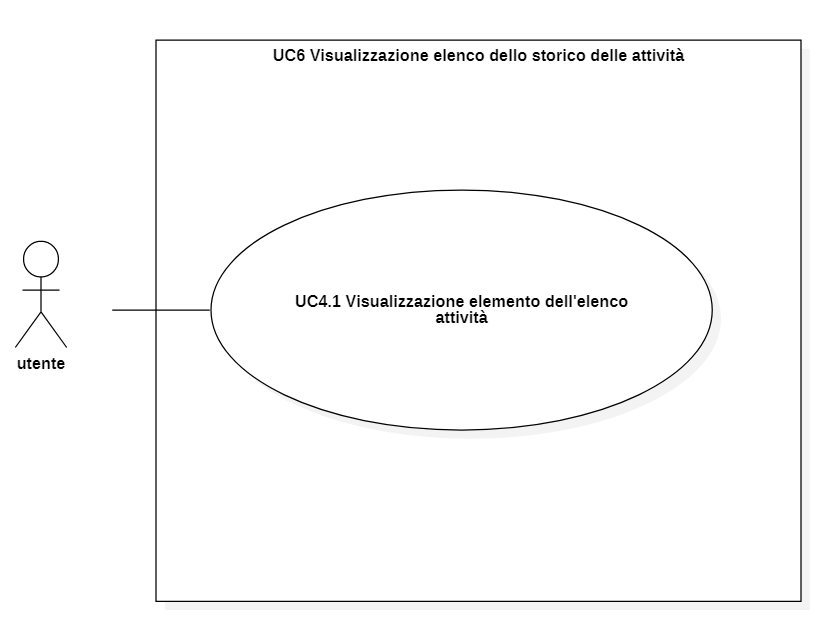
\includegraphics[width=0.8\linewidth]{res/images/UC6.png}
	\caption{Caso d'uso UC6 : visualizzazione elenco dello storico delle attività}
\end{figure}
\begin{itemize}
\item \textbf{Attori}: utente;
\item \textbf{Scopo e descrizione}: l’utente visualizza l'elenco dello storico delle attività sportive da lui pubblicate;
\item \textbf{Precondizione}: il sistema è pronto a ricevere richieste;
\item \textbf{Flusso principale degli eventi}:visualizzazione elemento dell'elenco attività(UC4.1);
\item \textbf{Postcondizione}: il sistema ha mostrato a schermo l'elenco dello storico delle attività.
\end{itemize}


\subsubsection{UC7 - Inserimento di un'attività}
\begin{figure}[H]
	\centering
	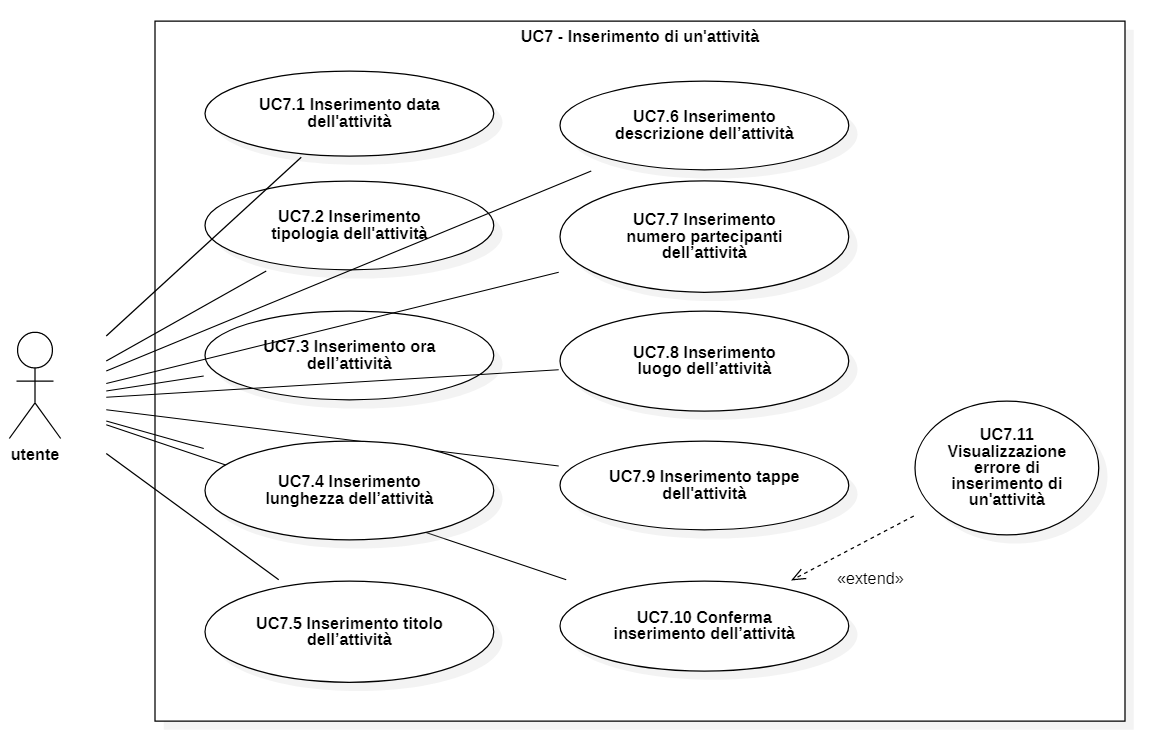
\includegraphics[width=0.8\linewidth]{res/images/UC7.png}
	\caption{Caso d'uso UC7 : Inserimento di un'attività}
\end{figure}
\begin{itemize}
	\item \textbf{Attori}: utente autenticato;
	\item \textbf{Scopo e descrizione}: l’utente vuole inserire una nuova attività;
	\item \textbf{Precondizione}: è pronto a ricevere i dati inseriti dall'utente;
	\item \textbf{Flusso principale degli eventi}:
	\begin{itemize}
		\item inserimento data dell’attività (UC7.1);
		\item inserimento tipologia dell’attività (UC7.2);
		\item inserimento ora dell’attività (UC7.3);
		\item inserimento lunghezza dell’attività (UC7.4);
		\item inserimento titolo dell’attività (UC7.5);
		\item inserimento descrizione dell’attività (UC7.6);
		\item inserimento numero partecipanti dell’attività (UC7.7);
		\item inserimento luogo dell’attività (UC7.8);
		\item inserimento tappe dell’attività (UC7.9);
		\item conferma inserimento dell’attività (UC7.10).
	\end{itemize}
\item \textbf{Estensioni}:
\begin{itemize}
	\item se l’utente inserisce dei dati non validi viene visualizzato l’errore di inserimento di un'attività (UC7.11 Visualizzazione errore di inserimento di un'attività);
\end{itemize}
	\item \textbf{Postcondizione}: l’utente ha inserito un'attività.
\end{itemize}

\subsubsection{UC7.1 - Inserimento data dell’attività }
\begin{itemize}
	\item \textbf{Attori}: utente autenticato;
	\item \textbf{Scopo e descrizione}: l’utente deve inserire la data dell'attività;
	\item \textbf{Precondizione}: il sistema è pronto a ricevere la data inserita dall’utente;
	\item \textbf{Flusso principale degli eventi}: l’utente digita la data;
	\item \textbf{Postcondizione}: l’utente ha inserito la data dell’attività.
\end{itemize}

\subsubsection{UC7.2 - Inserimento tipologia dell’attività}
\begin{itemize}
	\item \textbf{Attori}: utente autenticato;
	\item \textbf{Scopo e descrizione}: l’utente deve inserire la tipologia dell'attività;
	\item \textbf{Precondizione}: il sistema è pronto a ricevere la tipologia inserita dall’utente;
	\item \textbf{Flusso principale degli eventi}: l’utente digita il testo;
	\item \textbf{Postcondizione}: l’utente ha inserito la tipologia dell’attività.
\end{itemize}

\subsubsection{UC7.3 - Inserimento ora dell’attività }
\begin{itemize}
	\item \textbf{Attori}: utente autenticato;
	\item \textbf{Scopo e descrizione}: l’utente deve inserire l'ora dell'attività;
	\item \textbf{Precondizione}: il sistema è pronto a ricevere l'ora inserita dall’utente;
	\item \textbf{Flusso principale degli eventi}: l’utente digita l'ora;
	\item \textbf{Postcondizione}: l’utente ha inserito l'ora dell’attività.
\end{itemize}

\subsubsection{UC7.4 - Inserimento lunghezza dell’attività}
\begin{itemize}
	\item \textbf{Attori}: utente autenticato;
	\item \textbf{Scopo e descrizione}: l’utente deve inserire la lunghezza dell'attività espressa in km;
	\item \textbf{Precondizione}: il sistema è pronto a ricevere la lunghezza inserita dall’utente;
	\item \textbf{Flusso principale degli eventi}: l’utente digita il numero;
	\item \textbf{Postcondizione}: l’utente ha inserito la lunghezza dell’attività.
\end{itemize}

\subsubsection{UC7.5 - Inserimento titolo dell’attività }
\begin{itemize}
	\item \textbf{Attori}: utente autenticato;
	\item \textbf{Scopo e descrizione}: l’utente deve inserire il titolo dell'attività;
	\item \textbf{Precondizione}: il sistema è pronto a ricevere il titolo inserito dall’utente;
	\item \textbf{Flusso principale degli eventi}: l’utente digita il testo;
	\item \textbf{Postcondizione}: l’utente ha inserito il titolo dell’attività.
\end{itemize}

\subsubsection{UC7.6 - Inserimento descrizione dell’attività }
\begin{itemize}
	\item \textbf{Attori}: utente autenticato;
	\item \textbf{Scopo e descrizione}: l’utente deve inserire la descrizione dell'attività;
	\item \textbf{Precondizione}: il sistema è pronto a ricevere la descrizione inserita dall’utente;
	\item \textbf{Flusso principale degli eventi}: l’utente digita il testo;
	\item \textbf{Postcondizione}: l’utente ha inserito la descrizione dell’attività.
\end{itemize}


\subsubsection{UC7.7 - Inserimento numero partecipanti all’attività}
\begin{itemize}
	\item \textbf{Attori}: utente autenticato;
	\item \textbf{Scopo e descrizione}: l’utente deve inserire il numero partecipanti all'attività;
	\item \textbf{Precondizione}: il sistema è pronto a ricevere il numero inserito dall’utente;
	\item \textbf{Flusso principale degli eventi}: l’utente digita il numero;
	\item \textbf{Postcondizione}: l’utente ha inserito il numero partecipanti all’attività.
\end{itemize}
\subsubsection{UC7.8 - Inserimento luogo dell’attività }
\begin{itemize}
	\item \textbf{Attori}: utente autenticato;
	\item \textbf{Scopo e descrizione}: l’utente deve inserire il luogo in cui si svolge dell'attività;
	\item \textbf{Precondizione}: il sistema è pronto a ricevere il luogo inserito dall’utente;
	\item \textbf{Flusso principale degli eventi}: l’utente digita il testo;
	\item \textbf{Postcondizione}: l’utente ha inserito il luogo dell’attività.
\end{itemize}

\subsubsection{UC7.9 - Inserimento tappe dell’attività}
\begin{itemize}
	\item \textbf{Attori}: utente autenticato;
	\item \textbf{Scopo e descrizione}: l’utente deve inserire le tappe dell'attività;
	\item \textbf{Precondizione}: il sistema è pronto a ricevere le tappe inserite dall’utente;
	\item \textbf{Flusso principale degli eventi}: l’utente digita le tappe;
	\item \textbf{Postcondizione}: l’utente ha inserito le tappe dell'attività.
\end{itemize}

\subsubsection{UC7.10 - Conferma Inserimento dell'attività}
\begin{itemize}
	\item \textbf{Attori}: utente autenticato;
	\item \textbf{Scopo e descrizione}: l’utente deve confermare i dati inseriti durante la fase di inserimento di un'attività;
	\item \textbf{Precondizione}: il sistema mostra una schermata che permette all’utente di confermare i dati inseriti;
	\item \textbf{Flusso principale degli eventi}: l’utente conferma i dati inseriti;
	\item \textbf{Postcondizione}: l’utente ha confermato i dati inseriti e il sistema ha creato un'attività basandosi sui dati ottenuti.
\end{itemize}

\subsubsection{UC7.11 - Visualizzazione errore di inserimento di un'attività}
\begin{itemize}
	\item \textbf{Attori}: utente autenticato;
	\item \textbf{Scopo e descrizione}: l’utente ha inserito durante la fase di inserimento di un'attività dei dati non validi o nulli;
	\item \textbf{Precondizione}: l’utente ha inserito dei dati non validi per la creazione di un'attività;
	\item \textbf{Flusso principale degli eventi}: il sistema mostra a schermo un errore di inserimento di un'attività;
	\item \textbf{Postcondizione}: l’attività non viene creata e viene comunicato il messaggio di errore all’utente.
\end{itemize}

\subsubsection{UC8 - Modifica di un'attività}
\begin{itemize}
	\item \textbf{Attori}: utente autenticato;
	\item \textbf{Scopo e descrizione}: l’utente vuole modificare una attività precedentemente inserita;
	\item \textbf{Precondizione}: è pronto a ricevere le modifiche inserite dall'utente;
	\item \textbf{Flusso principale degli eventi}:l'utente modifica i dati desiderati;
	\item \textbf{Postcondizione}: il sistema ha modificato l'attività.
\end{itemize}

\subsubsection{UC9 - Eliminazione di un'attività}
\begin{itemize}
	\item \textbf{Attori}: utente autenticato;
	\item \textbf{Scopo e descrizione}: l’utente vuole eliminare una attività precedentemente inserita;
	\item \textbf{Precondizione}: è pronto a ricevere l'eliminazione di un'attività;
	\item \textbf{Flusso principale degli eventi}:l'utente seleziona l'attività da eliminare;
	\item \textbf{Postcondizione}: il sistema ha eliminato l'attività.
\end{itemize}